\chapter{相关研究综述}

本章系统综述与本文研究密切相关的已有工作。第\ref{sec:ch2-human}节聚焦三维人体重建，依次介绍参数化人体模型、基于神经辐射场（NeRF）的方法以及基于三维高斯溅射（3DGS）的方法，并分析可驱动数字人建模中的拓扑一致性问题，由此引出第三章的研究动机。第\ref{sec:ch2-garment}节聚焦三维服装建模与生成，回顾服装表示、几何重建路线和参数化制版路线，讨论多模态大模型在服装生成中的进展与不足，由此引出第四章的研究动机。第\ref{sec:ch2-summary}节给出本章小结。

\section{三维人体重建研究综述}
\label{sec:ch2-human}

三维人体重建旨在从图像、视频或深度传感器等观测数据中恢复数字人体模型，主要涉及人体形状、姿态与外观细节的重建。该任务在混合现实、远程通信、影视制作和医疗康复等场景中具有直接应用价值。本节从三维人体表示出发，依次综述基于参数化人体模型、NeRF和3DGS的方法，重点分析其在可驱动数字人建模中的能力与局限。

\subsection{参数化人体模型}
\label{subsec:ch2-parametric}

参数化人体模型是一种通过数学参数化方法对人体形态和运动特性进行抽象表征的计算模型，其核心思想是将人体的几何形变解耦为形状参数（描述体型差异）与姿态参数（描述关节运动）的联合函数。此类模型可以为三维人体重建提供稳定先验，是本文第三章和第四章的共同基础。本节先介绍主流参数化模型，再回顾基于这些模型的人体形状与姿态估计方法。

% ===== SMPL 系列模型 =====

\noindent\textbf{SMPL模型及其扩展}\enspace
SMPL（Skinned Multi-Person Linear Model）\cite{smpl}是目前应用最为广泛的参数化人体模型。该模型从大规模人体扫描数据中学习得到，通过体型参数$\boldsymbol{\beta} \in \mathbb{R}^{10}$和姿态参数$\boldsymbol{\theta} \in \mathbb{R}^{72}$两组低维向量控制人体网格的形状与姿态。具体而言，SMPL定义了一个包含$N=6890$个顶点和$M=13776$个三角面片的标准拓扑模板网格$\mathcal{M} = (\mathbf{V}, \mathbf{F})$，其顶点位置由以下函数确定：
\begin{equation}
    \mathbf{V}(\boldsymbol{\beta}, \boldsymbol{\theta}) = W\big(\bar{\mathbf{V}} + B_S(\boldsymbol{\beta}) + B_P(\boldsymbol{\theta}),\; \boldsymbol{\theta},\; \mathbf{W}\big),
    \label{eq:smpl}
\end{equation}
其中$\bar{\mathbf{V}} \in \mathbb{R}^{N \times 3}$为模板网格的均值形状，$B_S(\boldsymbol{\beta})$为体型混合形状函数（由主成分分析得到的线性基张成），$B_P(\boldsymbol{\theta})$为姿态依赖的形状修正项（补偿关节弯曲引起的局部形变），$W(\cdot)$表示线性混合蒙皮（Linear Blend Skinning, LBS）函数，$\mathbf{W} \in \mathbb{R}^{N \times K}$为预定义的蒙皮权重矩阵，$K=24$为骨骼关节数量。SMPL模型的核心优势在于：（a）低维参数化使其便于通过优化或回归从观测数据中估计；（b）固定拓扑结构提供了稳定的网格连接关系，为后续的纹理映射、物理仿真和高斯绑定等操作提供了天然的拓扑骨架；（c）LBS驱动机制使模型具备姿态可控性，支持任意姿态下的网格变形与动画生成。

在SMPL基础上，研究者提出了多种扩展模型。SMPL-X\cite{pavlakos2019expressive}增加了手部关节和面部表情参数，实现全身统一建模。SCAPE\cite{anguelov2005scape}采用基于三角形变换的非线性模型表达姿态形变。STAR\cite{osman2020star}通过稀疏训练策略提升模型紧凑性与泛化能力。FLAME\cite{li2017flame}则将类似思路扩展至人脸与头部建模。这些模型共同构成了当前参数化人体建模的基础。本文第三章以SMPL为拓扑骨架构建可变形穿衣人网格，第四章的人体测量先验提取同样依赖SMPL表示。
\begin{figure}[t]
    \centering
    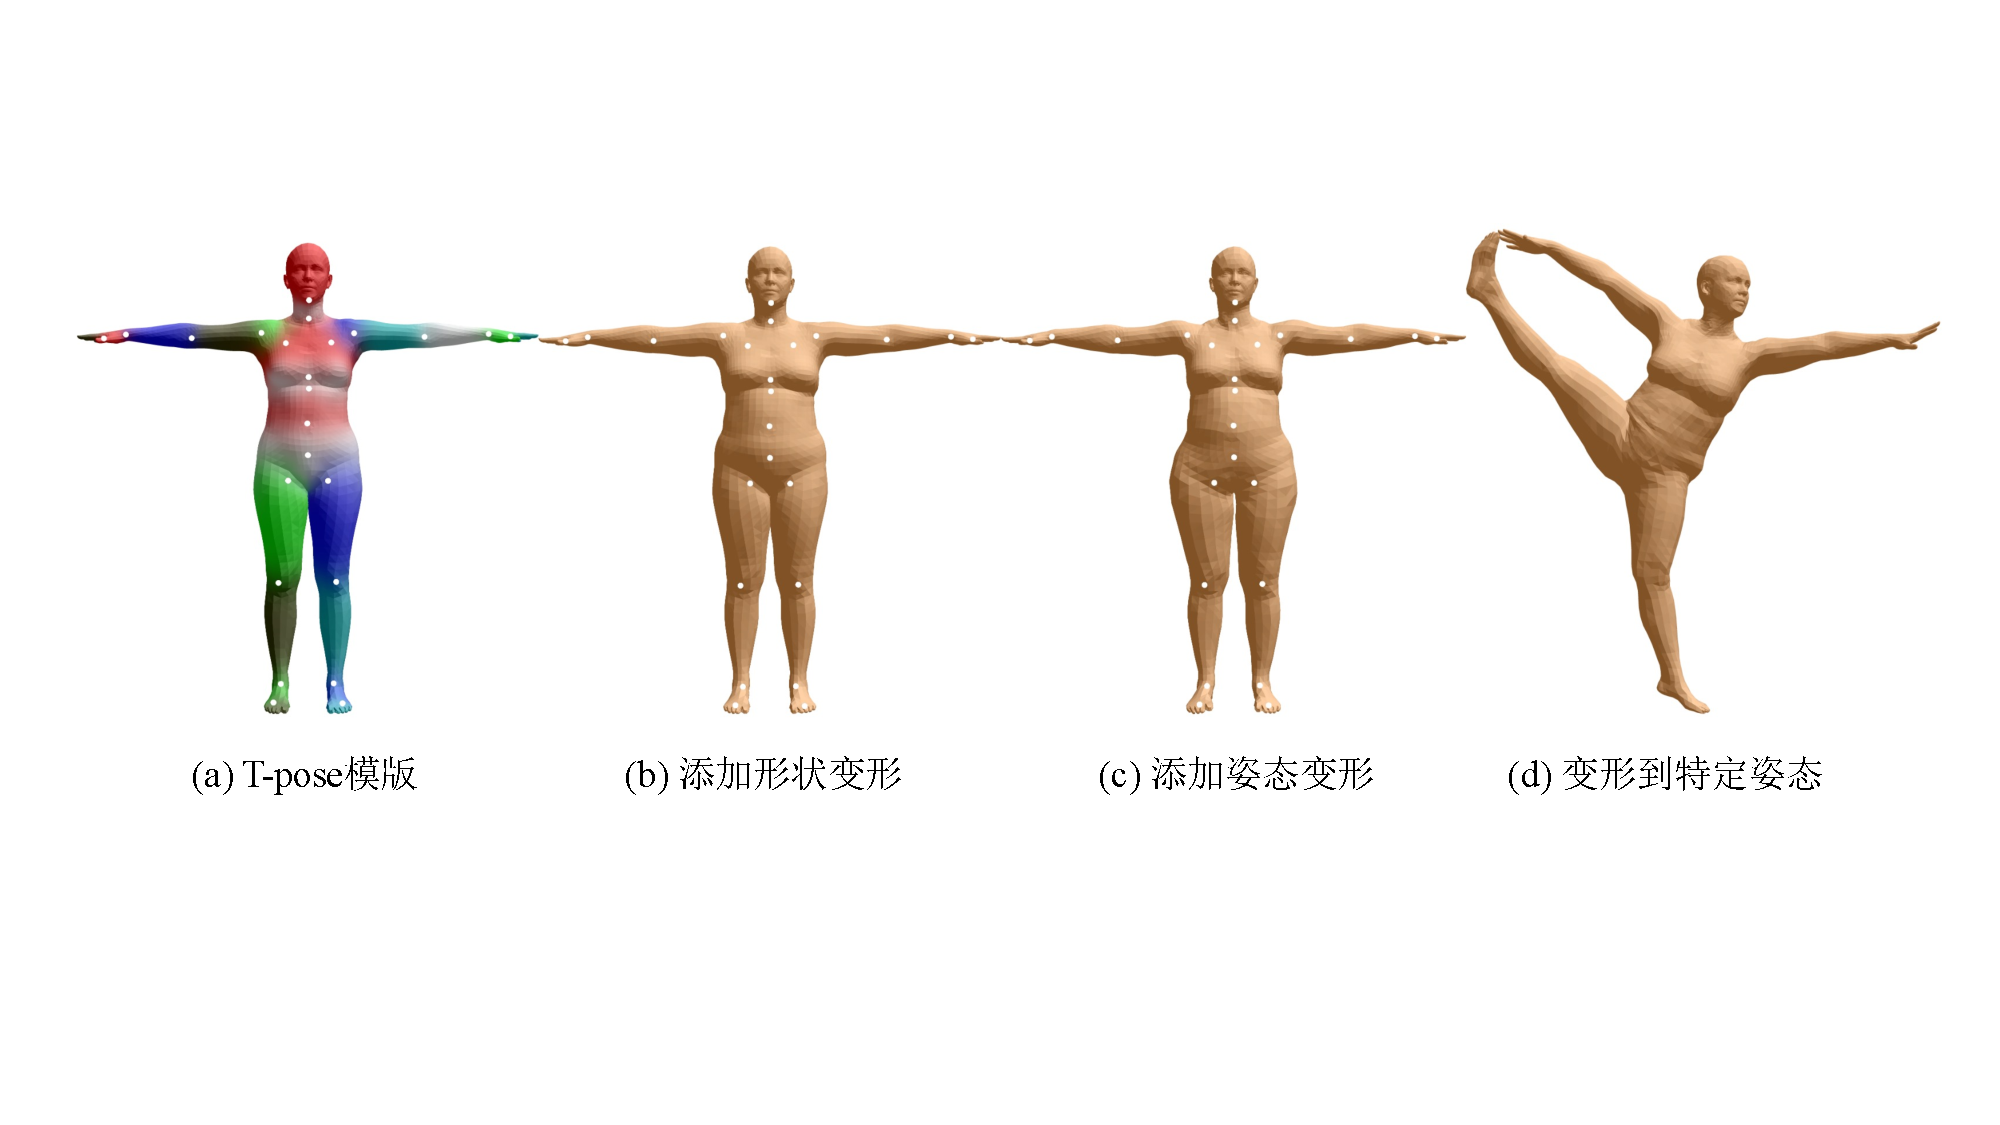
\includegraphics[width=\linewidth]{main/chapter2/figures/SMPL.pdf}
    \caption{SMPL参数化人体模型示意图\cite{smpl}}
    \label{fig:smpl}
\end{figure}

\subsection{基于神经辐射场的人体重建方法}
\label{subsec:ch2-nerf}

神经辐射场（Neural Radiance Fields, NeRF）\cite{nerf}为高保真三维重建与新视角合成提供了统一框架。NeRF 将场景表示为连续隐式函数 $F_{\Theta}: (\mathbf{x}, \mathbf{d}) \rightarrow (\mathbf{c}, \sigma)$，输入为空间坐标$\mathbf{x}$ 与视角方向 $\mathbf{d}$，输出颜色 $\mathbf{c}$ 与体积密度 $\sigma$。通过沿相机射线进行体渲染积分，NeRF 可从多视角图像学习场景表示并合成新视角图像。

% ===== NeRF在人体重建中的应用 =====

\noindent\textbf{NeRF与参数化模型的融合}\enspace
将NeRF用于动态人体重建的关键难点是运动建模。由于标准NeRF假设场景静态，现有方法通常借助SMPL提供骨骼运动学先验，将不同姿态的观测映射到统一的规范空间（Canonical Space），再在该空间学习静态辐射场。

Neural Body\cite{peng2021neural}是将神经辐射场与参数化人体模型结合的早期代表性工作。该方法在SMPL网格表面定义结构化可学习潜码（Latent Codes），并将其输入稀疏卷积网络（SparseConvNet）以生成潜码体（latent code volume），从而将原本定义在人体表面的离散特征扩散到邻近三维空间；随后对任意三维采样点，先从潜码体相邻体素顶点通过三线性插值获得该点潜特征，再输入MLP分别回归密度与颜色。这种“结构化潜码+体素扩散+点查询插值”的设计利用SMPL拓扑先验提升了空间特征的一致性，使模型能够在稀疏视角条件下合成连贯的人体外观。在此基础上，HumanNeRF\cite{weng2022humannerf}提出了“规范外观场+运动场”的统一优化框架：以视频帧为输入，在学习规范空间连续外观场的同时，学习从观测空间到规范空间的运动场映射；其中运动场被分解为由离散网格表示的骨骼刚性运动与由连续场表示的非刚性运动，从而分别刻画人体关节驱动与衣物等局部形变；此外，该方法对现成姿态估计器初始化的人体姿态进行联合细化以提升几何对齐精度，并在观测空间施加体渲染结果与输入图像之间的重建损失，驱动整体优化收敛到与观测一致的解。

\begin{figure}[t]
    \centering
    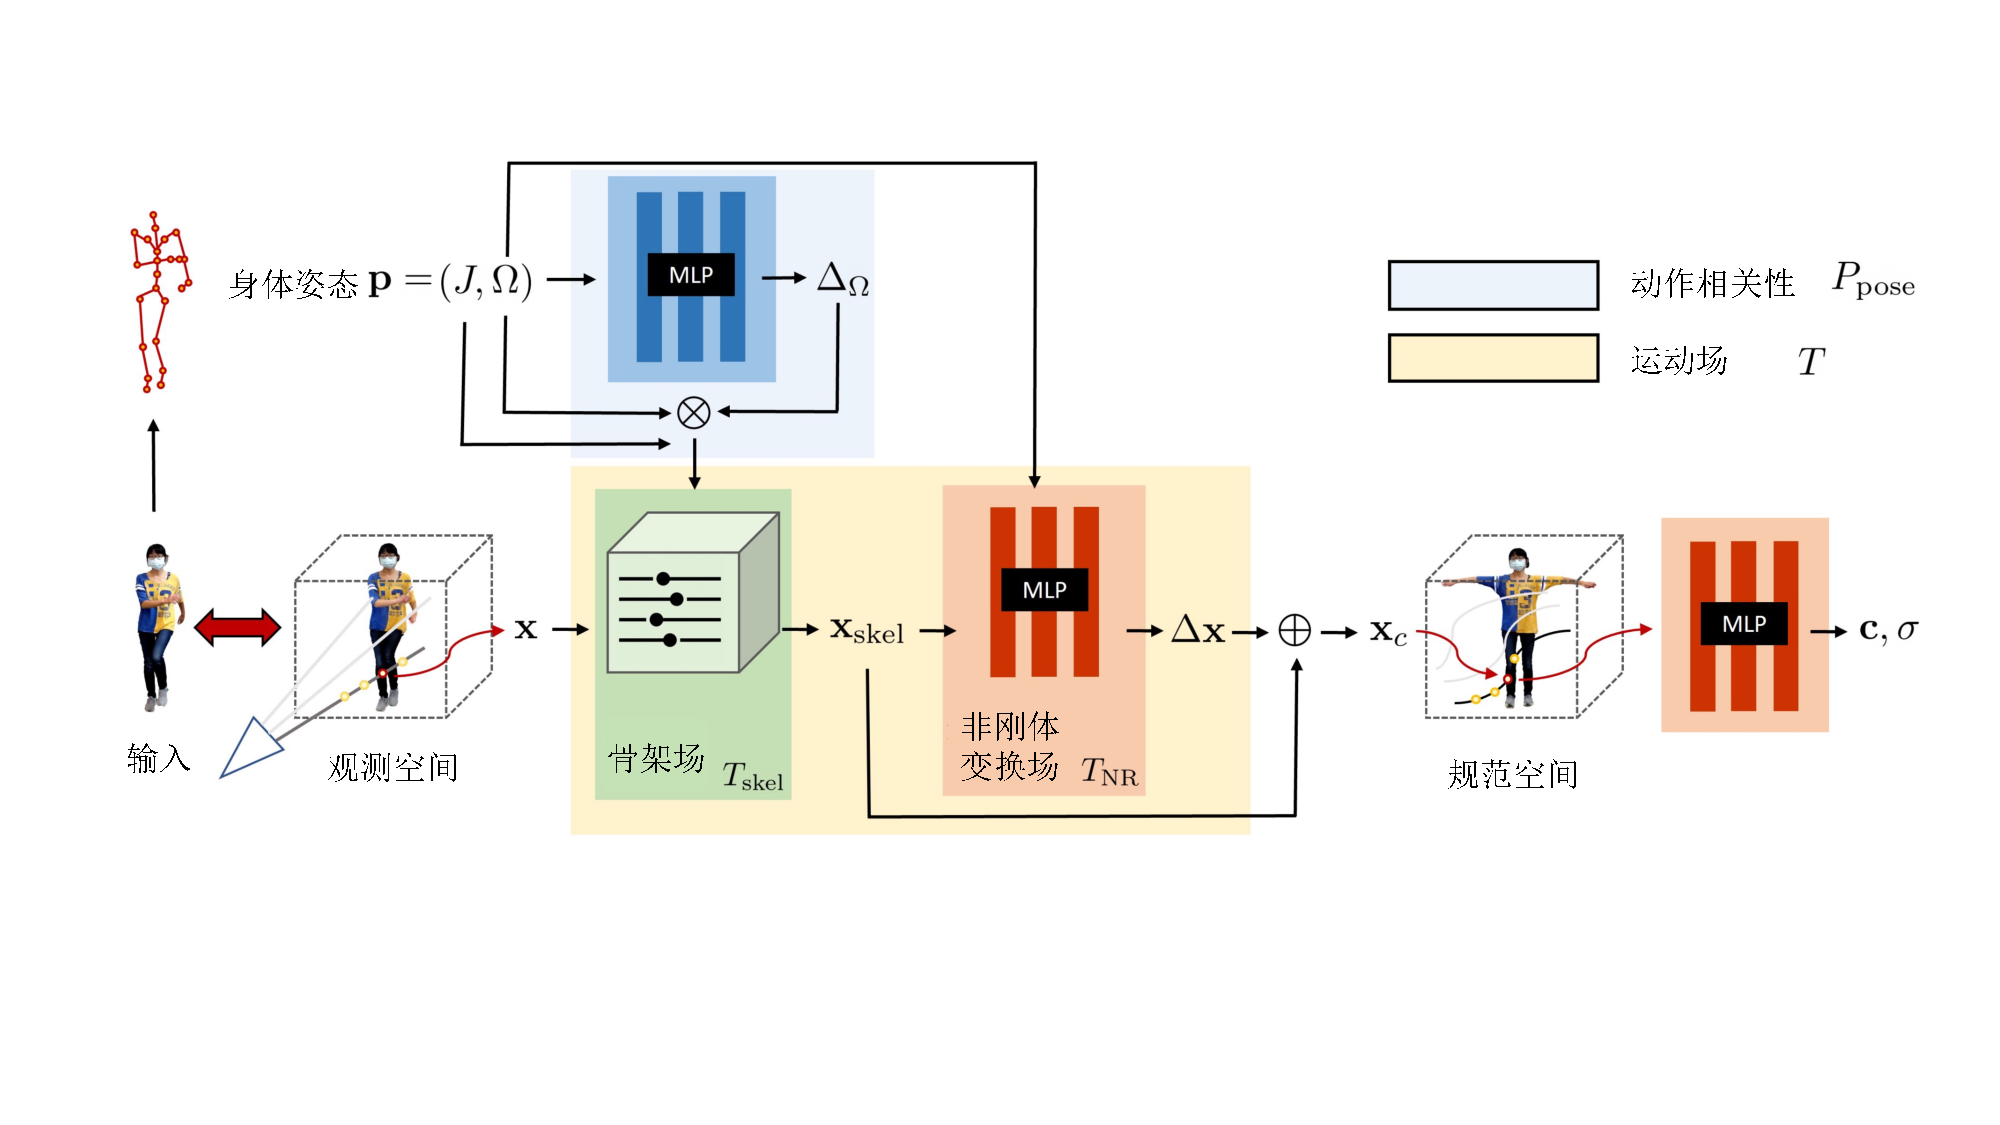
\includegraphics[width=\linewidth]{main/chapter2/figures/nerf-human.pdf}
    \caption{基于NeRF的典型人体重建方法流程示意}
    \label{fig:nerf-human}
\end{figure}

进一步地，MonoHuman\cite{yu2023monohuman}在HumanNeRF框架上构建共享双向形变机制：不同观测空间点先通过反向形变映射到统一规范空间，再由对称的前向形变回到观测空间，并通过一致性损失约束运动权重以提升跨帧对应稳定性；同时在前向对应搜索模块中，将规范空间点形变到两个对应空间以获取对应特征与颜色信息，再由Blend MLP生成的权重进行融合得到统一特征，用于引导最终渲染网络，从而提升时序一致性与几何保真度。与上述方法相比，Anim-NeRF\cite{anim-nerf}更强调基于视频序列的联合初始化与联合优化流程。该方法先估计逐帧相机参数与SMPL人体参数作为初始化，再在观测空间沿相机射线进行体渲染采样，并依据姿态引导形变将采样点映射至规范空间；随后由神经辐射场回归密度与颜色，经体渲染积分得到重建图像，并在人体掩码约束下最小化重建图像与真实图像误差，从而联合优化辐射场参数与逐帧人体参数。A-NeRF\cite{su2021anerf}则进一步提出了骨架驱动嵌入与模板无关神经表示相结合的可驱动人体建模方案：在学习用户专属神经人体模型的同时适配多样姿态，并在单视角或可用多视角条件下联合细化初始三维骨架姿态估计，从而减少对繁琐相机标定流程的依赖；其底层通过骨架条件编码与体渲染耦合，实现了关节化运动下外观与几何的一致重建。

\noindent\textbf{训练与推理加速}\enspace
标准NeRF训练与渲染都需要逐射线采样和MLP推理，计算开销高，训练常需数小时，单帧渲染常需数十秒。为缓解这一瓶颈，InstantAvatar\cite{instant-avatar}借鉴Instant-NGP\cite{mueller2022instant}的多分辨率哈希编码，将人体NeRF训练时间压缩到约60秒。Instant-NVR\cite{jiang2023instant}则面向人体-物体交互场景实现了即时体渲染重建。即便如此，NeRF方法仍依赖隐式体渲染管线，推理速度通常只有数帧每秒，难以满足实时交互，并且在分布外极端姿态下仍易出现伪影。

\noindent\textbf{局限性分析}\enspace
基于NeRF的人体重建方法在视觉保真度方面取得了显著进展，但仍面临以下固有局限：
（a）渲染效率不足：体渲染的逐像素射线采样机制导致渲染速度远低于实时要求，制约了在VR/AR等实时交互场景中的应用。
（b）几何表示的隐式性：NeRF以密度场隐式编码几何信息，难以直接提取显式网格或进行物理仿真，限制了其在下游应用中的灵活性。
（c）姿态泛化能力有限：依赖变形场将观测映射到规范空间的策略在大幅度未见姿态下容易出现映射失真，导致几何伪影。
上述局限推动了研究者向更高效的显式场景表示技术的探索。

\subsection{基于三维高斯溅射的人体重建方法}
\label{subsec:ch2-3dgs}

三维高斯溅射（3D Gaussian Splatting，3DGS）\cite{3dgs,YANG2026112923}是一种显式场景表示方法。与传统的隐式表示方法不同，3DGS利用三维高斯分布的特性将场景建模为一系列可学习的三维高斯体，并通过优化这些高斯体的参数捕捉场景的几何和外观信息。该方法以各向异性三维高斯基元建模场景，并通过可微光栅化实现高质量实时渲染。相比NeRF的隐式体渲染范式，3DGS在训练速度、渲染效率和显式可编辑性方面更有优势，已成为动态人体重建的重要技术路线。本节先介绍3DGS基本原理，再综述其在可驱动数字人中的应用，并分析现有方法的拓扑一致性问题。

\noindent\textbf{3DGS基本原理}\enspace
3DGS将场景表示为一组各向异性的三维高斯基元$\mathcal{G} = \{G_i\}_{i=1}^N$，每个高斯基元由中心位置$\boldsymbol{\mu}_i \in \mathbb{R}^3$、协方差矩阵$\boldsymbol{\Sigma}_i \in \mathbb{R}^{3 \times 3}$、不透明度$\alpha_i \in [0,1]$以及球谐系数$\mathbf{c}_i$参数化。为保证半正定性，协方差矩阵被分解为旋转矩阵$\mathbf{R}_i \in SO(3)$与缩放矩阵$\mathbf{S}_i$的乘积：$\boldsymbol{\Sigma}_i = \mathbf{R}_i \mathbf{S}_i \mathbf{S}_i^\top \mathbf{R}_i^\top$。渲染时，三维高斯经EWA投影变换\cite{zwicker2001ewa}映射至二维图像平面，像素颜色通过对深度排序后的高斯基元进行$\alpha$-blending累积得到：
\begin{equation}
    C(u) = \sum_{i \in \mathcal{N}} c_i \alpha_i' \prod_{j=1}^{i-1} (1 - \alpha_j'),
    \label{eq:ch2-3dgs-render}
\end{equation}
其中$c_i$为视角依赖的颜色，$\alpha_i'$为考虑像素位置处高斯概率密度后的有效不透明度。该光栅化过程完全可微，支持通过反向传播端到端优化所有高斯参数。3DGS在训练过程中还引入了自适应密度化策略，通过克隆与分裂操作动态调整高斯数量，以保证对场景细节的充分覆盖。

\noindent\textbf{3DGS在可驱动数字人建模中的应用}\enspace
将3DGS应用于可驱动人体建模时，核心问题在于如何将高斯基元与人体运动关联，使其能够跟随骨骼驱动进行合理的空间变形。现有方法普遍采用SMPL参数化模型作为运动学骨架，将高斯基元以不同方式“绑定”至人体网格或骨骼结构上，通过线性混合蒙皮驱动高斯基元的空间运动。根据高斯基元与网格拓扑之间的约束程度，可将现有工作分为以下几类：

\textbf{无约束优化方法}：以GaussianAvatar\cite{gaussian-avatar}、GART\cite{gart}、3DGS-Avatar\cite{qian20243dgs}和GauHuman\cite{hu2024gauhuman}为代表。这类方法将高斯的位置定义为相对于SMPL网格顶点的偏移，但旋转和缩放属性作为自由可学习参数，通过无约束的梯度下降进行优化。GaussianAvatar在每帧先拟合SMPL/SMPL-X人体并对其表面采样，将采样点写入UV位置图后经姿态编码器提取姿态特征，再与像素对齐的可优化特征张量融合，以学习人体粗粒度外观；随后通过高斯参数解码器预测各采样点的偏移、颜色与尺度参数，并与固定旋转和不透明度共同构成规范空间中的可驱动三维高斯；GART在规范空间以高斯混合显式表示可关节人体的形状与外观，并通过可学习蒙皮与潜在骨骼（latent bone）机制实现对高斯基元的高效姿态驱动，以刻画复杂非刚性形变；在渲染阶段采用高斯溅射进行高效可微渲染，并结合多种平滑正则项约束点式表示的局部连续性与稳定性；3DGS-Avatar则从SMPL表面采样初始化规范空间高斯，经由姿态条件非刚性形变模块对高斯进行衣物相关非刚性调整并产生姿态相关潜特征，再通过学习的神经蒙皮将其映射到观测空间，最后将高斯特征、姿态特征、逐帧潜码与视线方向输入小型MLP解码视角相关颜色，并通过可微高斯光栅化完成渲染；GauHuman以SMPL顶点初始化高斯中心，引入姿态细化模块与蒙皮权重场模块以学习从规范空间到姿态空间的蒙皮变换，并采用基于瓦片的可微光栅化实现高效渲染，同时结合人体先验与KL散度约束自适应调节高斯的分裂、克隆、合并与剪枝过程。这种无约束的优化策略虽然在训练姿态下能够获得较高的渲染质量，但容易导致高斯属性对训练姿态产生过拟合。当人体进入未见过的姿态时，高斯基元的旋转和缩放无法随网格的局部形变做出相应调整，表现为高斯基元脱离网格表面（“漂浮高斯”），产生表面空洞与几何伪影。图\ref{fig:gaussian-avatar}展示了GaussianAvatar的方法框架，作为该类方法的代表。

\begin{figure}[t]
    \centering
    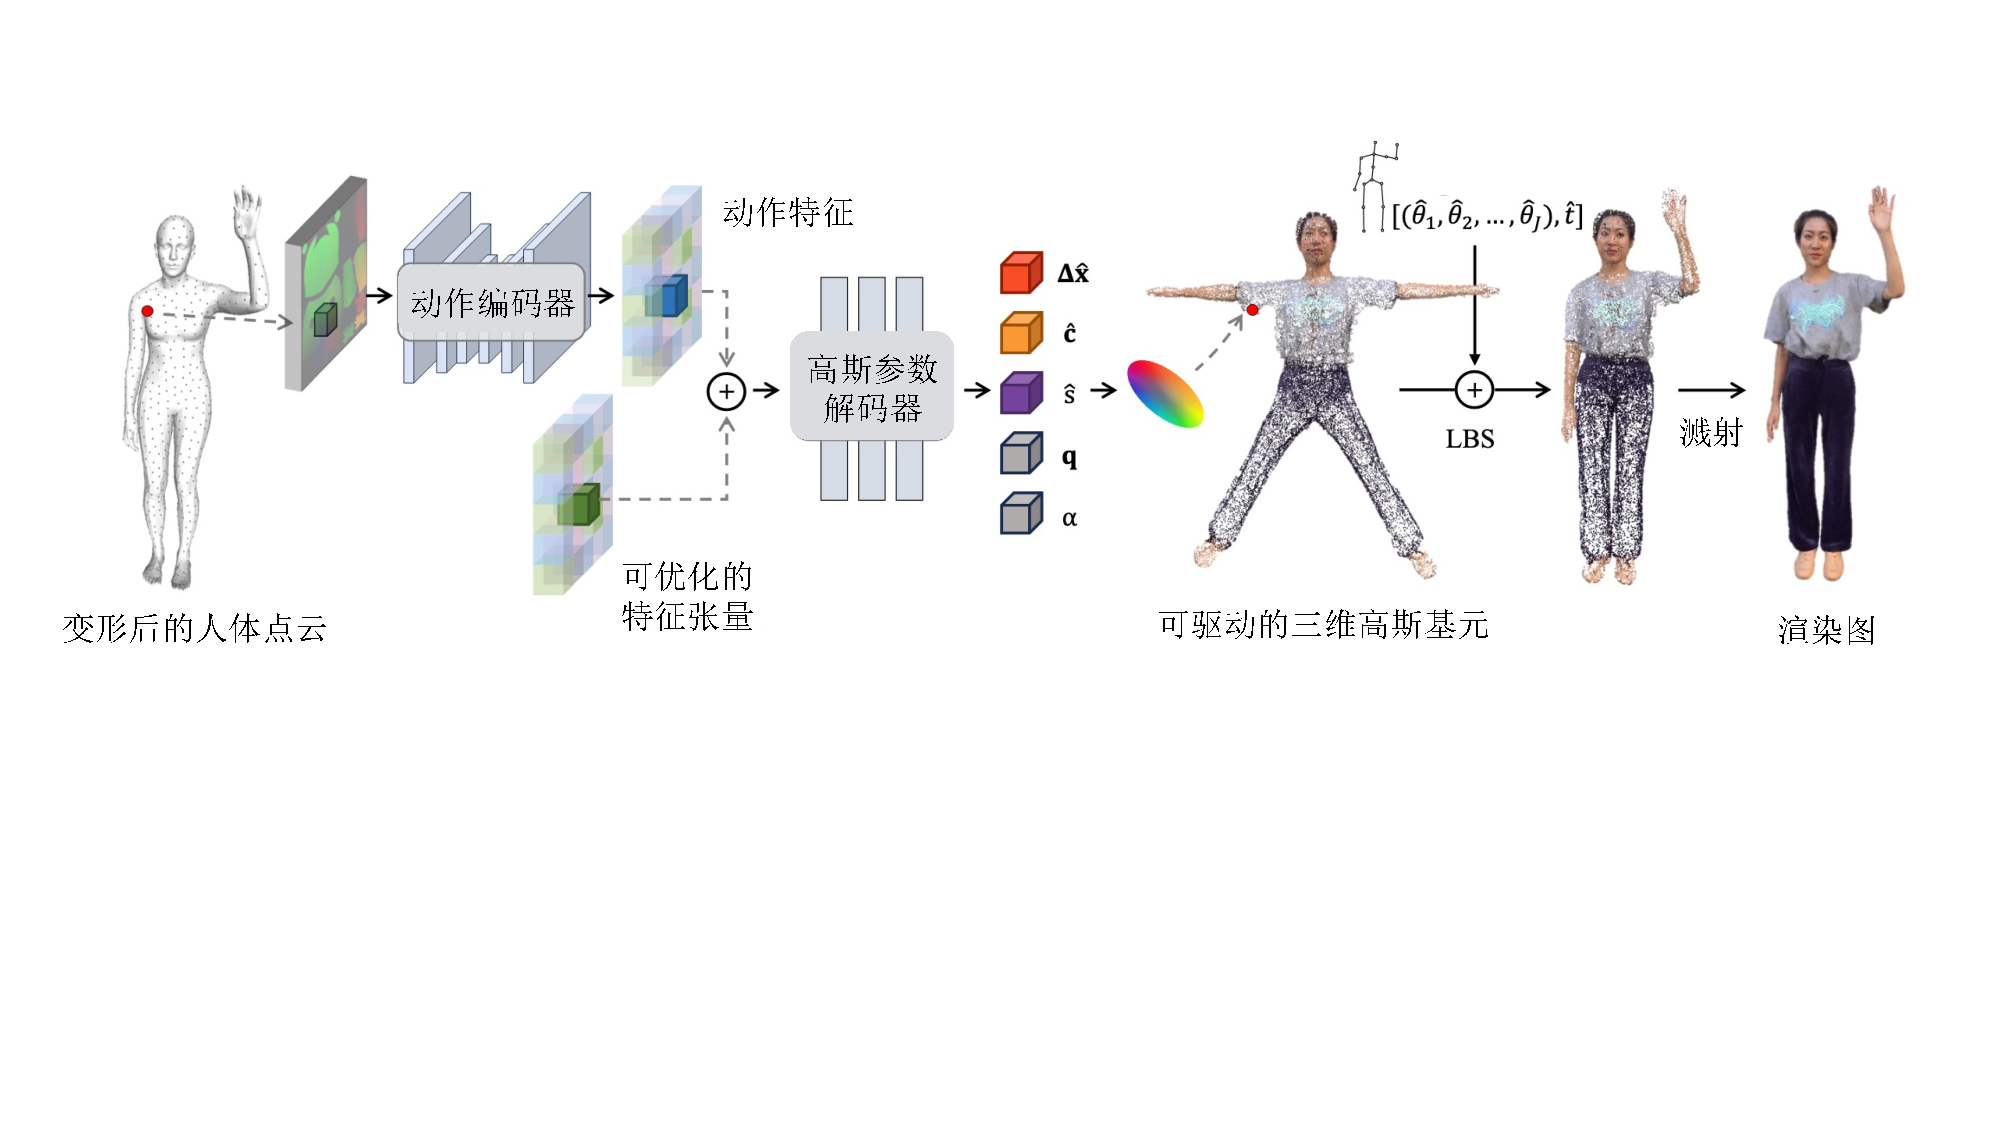
\includegraphics[width=\linewidth]{main/chapter2/figures/gaussianAvatar.pdf}
    \caption{GaussianAvatar方法框架示意图\cite{gaussian-avatar}}
    \label{fig:gaussian-avatar}
\end{figure}

\textbf{部分约束方法}：以IHuman\cite{ihuman}、GomAvatar\cite{gom-avatar}和SplattingAvatar\cite{shao2024splattingavatar}为代表。这类方法试图通过引入局部约束来增强高斯与网格之间的关联。IHuman利用网格面片法线约束高斯的旋转方向，使高斯朝向始终与局部表面一致，但其缩放属性仍作为自由变量优化，在大幅度形变下仍会出现覆盖范围与实际表面不匹配的问题。GomAvatar将高斯绑定至SMPL网格表面，通过重心坐标插值确定高斯位置，但缺乏对网格质量的正则化，当三角面片因驱动而退化为狭长形状时，高斯缩放会变得不稳定。SplattingAvatar提出了基于规范网格的高斯学习管线：在规范空间网格上学习带可训练嵌入的三维高斯，并利用网格的显式运动与形变将高斯映射到姿态空间进行可微光栅化；训练过程中同时优化高斯参数与嵌入参数。其位置由网格面片的重心点与沿插值法线方向的位移共同确定，并将姿态相关的旋转与尺度增量和姿态无关的旋转、尺度、不透明度与颜色联合建模，从而提升动态驱动下的外观表达能力。此外，SuGaR\cite{guedon2024sugar}通过表面对齐正则化将高斯分布约束到几何表面附近，并进一步支持高质量网格提取；HUGS\cite{kocabas2024hugs}通过前向蒙皮驱动与隐式特征参数化联合优化人物高斯，在单目场景下提升了人物重建的稳定性；Human Gaussian Splatting\cite{moreau2024human}则聚焦于可驱动人体的高效重建与渲染，通过人体先验引导高斯与表面结构对齐。也有工作将网格先验用于高斯的初始化\cite{waczynska2024games, qian2024gaussianavatars}，但上述方法在后续优化中均未能持续维持高斯与网格之间的拓扑一致性。

\noindent\textbf{现有方法的核心局限}\enspace
综合上述工作，当前3DGS可驱动人体方法的关键问题是：高斯几何属性（尤其旋转与缩放）与底层网格拓扑缺乏\textbf{显式解析关联}。人体表面的拉伸与压缩由网格拓扑关系决定。若高斯缩放不随局部形变同步变化，模型就更容易拟合训练姿态参数，而难以响应未见姿态下的真实表面变化，进而产生几何不一致。该问题直接构成了第三章的研究动机：将旋转与缩放由网格局部几何特征解析确定，以提升任意姿态下的几何一致性。

进一步地，这一问题本质上属于“表示自由度与物理约束不匹配”：当可学习参数自由度高于实际几何运动自由度时，模型会优先拟合训练分布中的外观误差，而非学习可迁移的几何规律。第三章引入拓扑绑定机制，针对这一结构性矛盾给出了约束化的解决方案。
\section{三维服装重建研究综述}
\label{sec:ch2-garment}

服装是数字人建模中的关键组成。在影视特效、虚拟试衣等场景中，服装模型不仅要外观真实，还要满足结构可编辑与物理可仿真。相较刚性物体或裸体人体，服装拓扑更复杂，褶皱与动力学变化更显著，因此三维重建与生成难度更高。该方向的发展大致经历了“直接几何重建—缝纫版型推断—参数化程序生成”三个阶段。本节按这一脉络综述主要方法，并分析现有方法在人体几何感知上的不足，由此引出第四章的研究动机。

\begin{figure}[b]
    \centering
    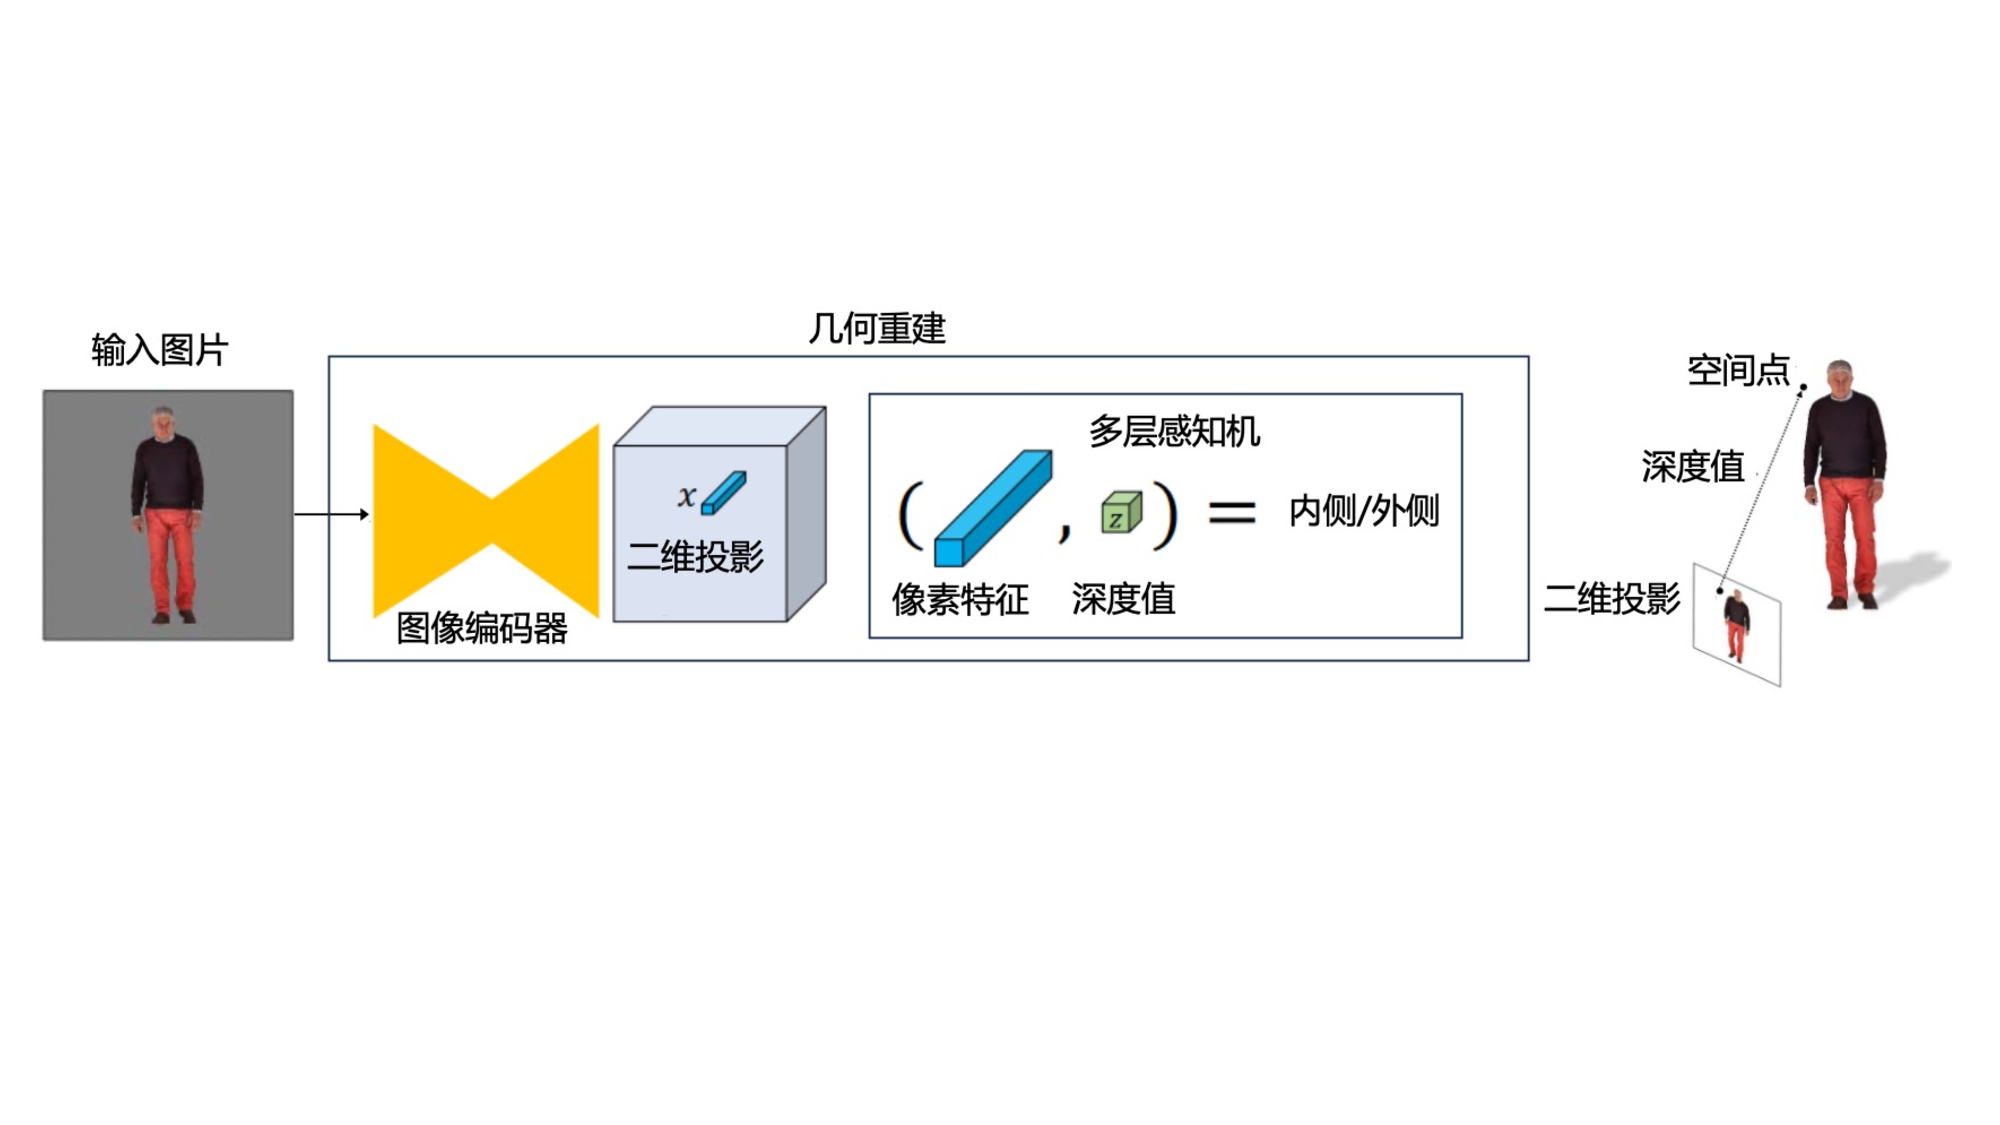
\includegraphics[width=\linewidth]{main/chapter2/figures/pifu.pdf}
    \caption{PIFu方法框架示意图\cite{saito2019pifu}}
    \label{fig:pifu}
\end{figure}

\subsection{基于显式几何重建的服装建模方法}

基于显式几何重建的方法直接从图像回归或优化服装三维几何（如网格、点云或高斯基元），重点提升外观保真度与几何一致性。按技术路径可将其概括为三类：基于隐式场的无模板方法、基于模板与形变的分层方法，以及基于三维高斯溅射的高保真方法。

\noindent\textbf{基于隐式场的无模板方法} \enspace
无模板方法不依赖底层参数化人体模型，直接从图像中推断穿衣人体的完整三维几何。PIFu 系列工作成为该领域的里程碑：PIFu\cite{saito2019pifu}提出像素对齐隐式函数，将二维图像特征与三维坐标深度融合，实现单图高保真重建，图\ref{fig:pifu}展示了 PIFu 的网络结构；StereoPIFu\cite{yang2021stereopifu} 引入双目视差特征，有效缓解深度歧义问题并恢复绝对尺度；PIFuHD\cite{saito2020pifuhd}进一步融合高分辨率的法向预测网络，在褶皱、衣纹等细节上实现更高精度的重建。针对 MLP 难以捕捉高频信号的缺陷，研究者提出多种改进方案。例如，位置编码方法\cite{nerf, tancik2020fourfeat}通过对输入坐标进行傅里叶变换注入高频信息，SIREN\cite{sitzmann2019siren}则采用周期性正弦激活函数增强网络表达能力，显著提升了曲面光滑度与细节还原能力。SiCloPe\cite{8954112}通过合成多视角轮廓图优化隐式场推理，但在凹形区域一致性上仍存在局限。Li\cite{li2020monoport}等人则提出实时重建框架，结合多尺度表面定位与直接渲染技术，首次实现了单目视频流中动态隐式场的在线生成。总体而言，该路线在几何重建精度与细节表达上持续提升，但仍主要面向整体穿衣人体重建，缺乏对服装语义的独立建模，因此在换装与物理仿真等下游任务中仍受限制。

\noindent\textbf{基于模板与形变的分层方法}\enspace
为实现人体与服装的解耦建模，另一类方法利用SMPL等参数化模型作为底层先验，将服装表示为人体表面的位移场或独立图层。早期的SMPL+D方案\cite{alldieck2019tex2shape}通过在SMPL网格顶点上添加位移向量来表示贴身衣物，但受限于SMPL的固定拓扑，无法表达裙子、大衣等与人体拓扑不同的宽松服装。TailorNet\cite{patel2020tailornet}在此基础上提出了低频与高频形变分解策略：先由统一模型预测与体型和风格相关的低频服装形变，再对若干原型体型-风格对的姿态相关高频细节分别建模，并通过RBF核进行加权混合；最终将低频与高频结果相加得到未姿态化服装，再通过标准蒙皮得到目标姿态下的服装形状。Multi-Garment Net\cite{bhatnagar2019mgn}首次将服装从人体网格中分离为独立图层，分别建模上衣和裤子，初步实现了服装的参数化表达。BCNet\cite{jiang2020bcnet}提出了一种更为解耦的方案：该方法通过独立的图卷积网络预测服装自适应的蒙皮权重，打破了服装与人体在蒙皮权重上的硬绑定约束，使模型能够联合重建人体和具有独立运动模式的宽松服装，并支持跨图像的换装与姿态重定向。Garment3DGen\cite{sarafianos2024garment3dgen}则利用图像到三维扩散模型生成粗略几何作为伪真值，通过可微渲染优化基础模板网格，实现了从单图到三维服装的形变迁移。

SMPLicit\cite{corona2021smplicit}在训练阶段以隐式函数网络学习查询点到服装表面的无符号距离场值，并结合由SMPL遮挡图编码得到的裁片形状潜变量与auto-decoder风格潜变量联合建模服装潜在空间。在推理阶段，该方法对三维空间进行密集采样，并通过Marching Cubes提取服装网格，随后利用最近SMPL顶点的学习蒙皮参数完成服装姿态驱动。DrapeNet\cite{de2023drapenet}采用生成网络与悬垂网络协同的两阶段框架：前者将服装嵌入紧凑潜变量并预测对应的无符号距离场，再通过等值面提取恢复几何；后者以该潜变量为条件，在自监督训练下预测作用于输入服装与规范参考服装顶点的位移场，并结合预测的蒙皮权重与人体体型、姿态参数完成服装姿态化驱动。该方法还引入交叠消解模块以抑制上下装之间的几何穿插，从而提升多层服装重建稳定性。

\noindent\textbf{基于三维高斯溅射的高保真方法}\enspace
传统网格加贴图的表示方式难以逼真地表达毛发、薄纱等复杂材质以及精细的光照变化。近年来，三维高斯溅射技术为服装的高保真重建提供了新的解决方案。Animatable Gaussians\cite{li2024animatablegaussians}将3DGS应用于动态穿衣人体建模，通过学习与姿态相关的高斯特征图实现实时渲染，但其服装与人体耦合为整体，无法将衣物作为独立资产提取。Gaussian Garments\cite{rong2024gaussian}提出了一种三维网格与三维高斯纹理紧密耦合的服装表示方法：在几何层面以网格表达服装的结构与拓扑，在外观层面以附着于网格表面的高斯基元编码高保真的纹理细节（包括毛发等高频特征）。该方法还通过微调图神经网络模拟真实布料的物理运动规律，使提取的服装具备独立的可仿真性，支持重定向、缩放与多层叠穿。


\noindent\textbf{局限性分析}\enspace
尽管显式几何重建方法在视觉效果上表现较好，但多数方法的输出仍以整体网格、点云或高斯集合为主，缺少缝纫版型结构与物理裁片属性。若要在工业软件中进行二次仿真或款式编辑，仍需较多人工后处理。这些局限性表明，显式几何重建方法更适用于单纯的视觉内容展示与离线资产制作，难以满足数字服装在“可仿真、可编辑、可制造”等工业级任务上的需求。这一痛点推动了后续研究从纯几何重建路线转向基于缝纫版型特征的结构化生成路线。

\subsection{基于缝纫版型的服装重建方法}

真实服装由二维裁片缝合而成。直接推断二维缝纫版型更符合制造过程，也更易接入物理仿真引擎，从而避免几何重建中常见的拓扑不合法问题。

\begin{figure}[t]
    \centering
    \includegraphics[width=\linewidth]{main/chapter2/figures/sewFormer.pdf}
    \caption{SewFormer方法框架示意图\cite{liu2023sewformer}}
    \label{fig:sewformer}
\end{figure}

\noindent\textbf{基于三维输入的版型推断}\enspace
早期方法多依赖三维点云或网格作为输入。NeuralTailor\cite{korosteleva2022neuraltailor}是该方向的代表性工作，该方法先通过两层EdgeConv提取逐点特征，并经平均池化得到全局服装潜在表示；随后采用层次化LSTM解码，先由版片级LSTM展开各版片编码，再由版片内部LSTM生成边序列特征（含缝合信息）与版片六维放置信息，最终恢复结构化缝纫版型。该方法验证了“点云编码+序列化版型解码”的可行性，但对输入三维数据质量和完整性依赖较强，难以直接从单张图像进行端到端推断。

\noindent\textbf{基于单张图像的版型重建}\enspace
如图\ref{fig:sewformer}所示，SewFormer\cite{liu2023sewformer}提出了首个仅需单张野外图像即可重建二维缝纫版型的端到端框架。该方法先将输入图像送入视觉编码器，得到序列化视觉token；随后通过两级Transformer解码器依次生成布片级与边缘级特征token，用于恢复各个服装裁片的几何结构；在此基础上，边缘特征进一步输入缝合关系预测模块，以估计裁片边之间的缝合对应关系。该方法同时引入了基于SMPL人体先验的正则化损失与新型形状损失。结合其构建的百万级合成数据集SewFactory，SewFormer在面对复杂人体姿态和真实照片时展现了较强的版型预测精度与拓扑正确性。

\noindent\textbf{局限性分析}\enspace
基于深度学习直接回归版型坐标的方法存在精度瓶颈。网络在回归高精度几何坐标时容易产生数值偏差，在长尾样本上更易输出拓扑错误版型（如多边形自交、面板缺失），进而导致物理悬垂仿真失败。该瓶颈说明，仅通过增加网络容量并不能从根本上解决版型合法性问题。若输出空间本身缺乏结构约束，模型在分布外输入下仍可能产生不可执行结果。因此，需要在表示层面引入“先保证合法，再优化精度”的生成机制。这一问题促使研究者进一步探索参数化和程序化生成路线。

\subsection{基于参数化程序的服装生成方法}

为解决直接回归坐标带来的拓扑合法性问题，研究者提出了参数化与程序化服装生成范式。该范式不直接预测版型坐标，而是调整预定义模板中的控制参数，由规则系统确定性生成服装版型，从机制上保障拓扑正确性。

\noindent\textbf{参数化制版框架}\enspace
GarmentCode\cite{GarmentCode2023}是该方向的奠基性工作，提出了一种面向参数化缝纫版型的领域特定语言（DSL）。通过层次化的配置文件即可精确定义服装组件的类型、尺寸与缝合规则，一段程序化配置经解析器解释后可确定性地生成拓扑合法的二维版型及对应的三维服装。这种表示方式不仅紧凑、语义明确，还为后续基于大语言模型的服装生成奠定了技术基础。GarmentCodeData\cite{GarmentCodeData:2024}进一步构建了大规模参数化服装数据集以支持模型训练与评估。

\noindent\textbf{多模态大模型驱动的参数化生成}\enspace
随着多模态大模型（Large Multimodal Models, LMMs）的快速发展，学术界开始探索利用其视觉理解与代码合成能力，直接从文本或图像生成参数化服装代码。DressCode\cite{he2024dresscode}采用SewingGPT管线，将缝纫版型量化为离散token序列，并以GPT架构进行自回归生成，在文本提示词引导下生成具有较高多样性与质量的版型结果。Design2GarmentCode\cite{zhou2025design2garmentcode}提出了一种神经符号方法，将服装生成视为程序合成任务：首先使用多模态理解代理提取图像中的几何与拓扑特征，再通过微调的领域特定语言生成代理将特征转化为精确的GarmentCode代码，在结构准确性与跨模态泛化能力上表现优异。其整体流程如图\ref{fig:d2gc}所示。ChatGarment\cite{bian2024chatgarment}基于LLaVA\cite{liu2023llava}架构进行微调，使其能够接受图文多模态输入并直接输出包含服装几何结构与连续数值尺寸的结构化JSON配置文件，还支持多轮对话式的局部交互编辑。

\begin{figure}[htbp]
    \centering
    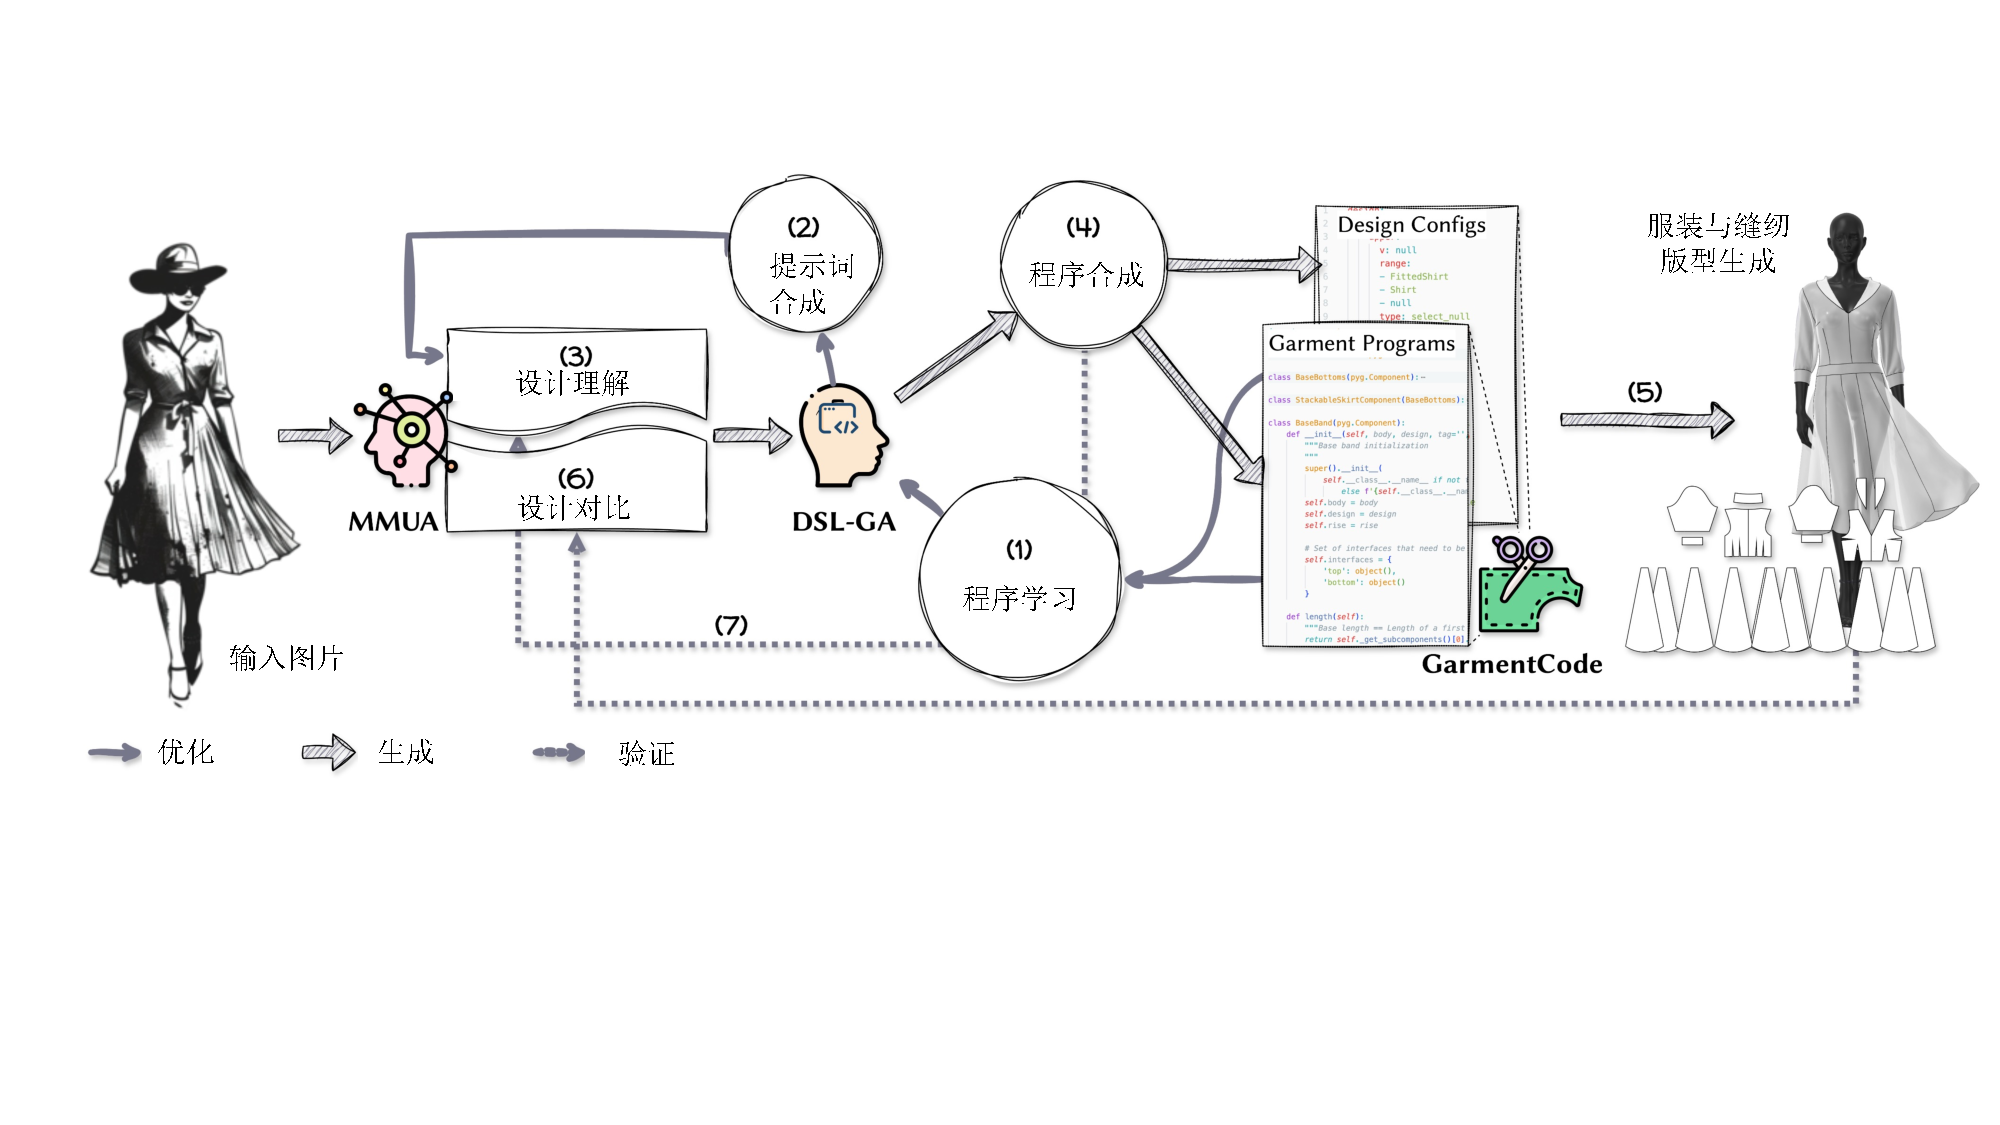
\includegraphics[width=\linewidth]{main/chapter2/figures/d2g.pdf}
    \caption{Design2GarmentCode方法框架示意图\cite{zhou2025design2garmentcode}}
    \label{fig:d2gc}
\end{figure}

\noindent\textbf{当前方法面临的核心挑战}\enspace
尽管大模型在离散属性预测（如款式类型、是否有衣领）上效果较好，但在连续物理尺寸预测上仍有明显偏差。从二维像素直接回归三维绝对尺寸（如衣长65 cm）本质上属于不适定问题。现有方法为此做出妥协：Design2GarmentCode将连续尺寸离散化为多选项（如“全长”“半长”），以精度换稳定；ChatGarment通过额外标志符和投影层处理连续回归，带来更高的微调与标注成本。

上述方法在尺寸预测中普遍忽略了一个关键物理前提，即\textbf{人体几何先验}。服装尺寸与人体参数直接相关：袖长对应臂长，裙长对应腿长，胸围对应体围。若生成过程不引入人体尺度作为参照，仅依靠图像像素拟合绝对尺寸，本质上属于约束不足的不适定问题。该分析直接构成第四章的研究动机：将SMPL编码的身体测量信息作为显式几何先验注入推理过程，把绝对尺寸预测转化为基于人体先验的比例推理，从而在无需额外训练回归网络的前提下提高参数精度与体型匹配度。

\section{本章小结}
\label{sec:ch2-summary}

本章围绕三维人体重建与三维服装重建两个方向，系统梳理了相关理论基础与研究现状。综述内容覆盖了从数字人表示方式、服装建模范式到关键技术瓶颈的发展脉络，为后续的问题定义与方法设计提供了依据。通过横向比较各类方法的优劣，明确了本文研究的切入点。

在三维人体重建方面，本章综述了参数化人体模型、NeRF方法和3DGS方法。分析表明，现有3DGS可驱动人体方法中，高斯几何属性与底层网格拓扑缺乏显式解析关联，导致模型在分布外姿态下出现明显几何不一致。这一问题构成了第三章的研究动机。基于该结论，第三章将重点讨论如何通过拓扑绑定机制建立高斯属性与网格局部几何之间的稳定映射，以提升可驱动人体在复杂姿态下的几何一致性与渲染稳定性。

在三维服装重建方面，本章沿“显式几何重建—缝纫版型推断—参数化程序生成”的脉络梳理了各阶段方法。分析表明，当前基于多模态大模型的参数化服装生成方法在拓扑正确性与泛化能力上已有进展，但在连续物理尺寸预测上仍存在不足：缺乏人体几何显式感知，导致版型绝对尺寸与体型不匹配。现有妥协方案（如尺寸离散化、额外训练回归网络）未从根源解决该问题。基于此，第四章将SMPL编码的身体测量信息作为几何先验注入推理过程，以缓解尺寸预测的不适定性问题。该设计与第三章在“几何先验显式化”上的思路保持一致。